\documentclass[12pt,a4paper]{article}

% To use this template make changes to following:
% 1. Fill-ables section.
% 2. Instructions.
% 3. Marks table.
% 4. Actual questions.

% ================================ 1. Fill-ables ================================
\newcommand\University{National University of Computer and Emerging Sciences}
\newcommand\Department{School of Engineering}
\newcommand\Campus{Islamabad Campus}
\newcommand\Semester{Fall 2014}
\newcommand\Exam{Sessional -- I}
\newcommand\Subject{EE305--Electromagnetic Theory}
\newcommand\ExamDate{Saturday, September 27, 2014}
\newcommand\InstructorOne{Attique Dawood}
\newcommand\InstructorTwo{\null~}
\newcommand\InstructorThree{\null}
\newcommand\TotalTime{01 Hour}
\newcommand\TotalMarks{50}
\newcommand\TotalQuestions{5}
\newcommand\TotalPages{\pageref{LastPage}} % Automatic: No need to change this.
% Marks of each question
\def\Qone{10}
\def\Qtwo{10}
\def\Qthree{10}
\def\Qfour{10}
\def\Qfive{10}
\def\Qsix{0}
\def\Qseven{0}
\def\Qeight{0}
\def\Qnine{0}
\def\Qten{0}
% ============================================================================

% ============== 2. Packages ==============
\usepackage{amsmath}
\usepackage{float}
\usepackage{graphicx}
\usepackage[hyphens]{url}
\usepackage[hidelinks]{hyperref}	% Clickable links to figures, references and urls.
\usepackage{lastpage}
\usepackage{array}
\usepackage{fancyhdr}
\usepackage{afterpage}
% Drawing packages.
\usepackage{pgf}
\usepackage{tikz}
% Listings for formatting code.
\usepackage{listings}
\usepackage{textcomp}

% General listings options.
\lstset{breaklines=true, basicstyle=\footnotesize\ttfamily, tabsize=4, numbers=left, stepnumber=1, frame=none, showstringspaces=false, upquote=true}
% C++ specific high-lighting. Comments are 50/50 shades of green/black and strings coloured with 60/40 red/black mixture.
\lstset{language=[ISO]C++, commentstyle=\color{green!50!black}, keywordstyle=\color{blue}, stringstyle=\color{red!60!black}}

% Table cell alignment directives.
\newcolumntype{L}[1]{>{\raggedright\let\newline\\\arraybackslash\hspace{0pt}}m{#1}}
\newcolumntype{C}[1]{>{\centering\let\newline\\\arraybackslash\hspace{0pt}}m{#1}}
\newcolumntype{R}[1]{>{\raggedleft\let\newline\\\arraybackslash\hspace{0pt}}m{#1}}

% Line spacing.
\def\SingleSpacing{\def\baselinestretch{1}\large\normalsize}
\def\DoubleSpacing{\def\baselinestretch{1.5}\large\normalsize}

% Margins.
\setlength{\oddsidemargin}{0in}
\setlength{\evensidemargin}{0in}
\setlength{\headheight}{28pt}
\setlength{\headsep}{2.5pt}
\setlength{\topmargin}{-60pt}
\setlength{\textwidth}{6.5in}
\setlength{\textheight}{10.75in} % Actual: 10.75in

% ============================= 3. Header and Footer ============================
\pagestyle{empty}
% Header
\chead
{
	{\large\textbf{\University}}\\
	\begin{minipage}{0.45\textwidth}
	\begin{center}
	{\small\textbf{\Department}}
	\end{center}
	\end{minipage}
	\begin{minipage}{0.45\textwidth}
	\begin{center}
	{\small\textbf{\Campus}}
	\end{center}
	\end{minipage}
}
% Footer
\lfoot{{\small\Exam}}
\cfoot{{\small\Semester}}
\rfoot{{\small Page \textbf{\thepage}~of \textbf{\TotalPages}}}
\renewcommand{\headrulewidth}{0.4pt}
\renewcommand{\footrulewidth}{0.4pt}
% ================================= 4. Front Page ===============================
\begin{document}
% A cute macro to add up marks of all individual questions. Uncomment if you want to use this.
\pgfmathtruncatemacro\TotalMarks{\Qone+\Qtwo+\Qthree+\Qfour+\Qfive+\Qsix+\Qseven+\Qeight+\Qnine+\Qten}
% Use this macro if marks are in decimal points
%\newcommand\TotalMarks{\pgfmathsetmacro\TotalMarks{\Qone+\Qtwo+\Qthree+\Qfour+\Qfive+\Qsix+\Qseven+\Qeight+\Qnine+\Qten}}
\begin{minipage}[t]{0.6\textwidth}
\begin{flushleft}
\DoubleSpacing
{\Large\textbf{\Subject}}\\
{\normalsize\ExamDate}\\
{\large\textbf{Course Instructor}}\\
{\normalsize\InstructorOne}\\
{\normalsize\InstructorTwo}\\
{\normalsize\InstructorThree}
\end{flushleft}
\end{minipage}
\begin{minipage}[t]{0.01\textwidth}
~
\end{minipage}
\begin{minipage}[t]{0.325\textwidth}
\DoubleSpacing
{\normalsize Serial No:}\\
{\Large\textbf{\Exam}}\\
{\large\textbf{Total Time: \TotalTime}}\\
{\large\textbf{Total Marks: \TotalMarks}}\\[1cm]
\rule{5cm}{0.2mm}\\[-0.25cm]
{\small Signature of Invigilator}
\end{minipage}
\SingleSpacing
~\\[1.5cm] % Extra space.
\rule{7cm}{0.2mm}~\rule{2.5cm}{0.2mm}~\rule{2cm}{0.2mm}~\rule{4.5cm}{0.2mm}\\
{\small Student Name\hspace{4.75cm}Roll No\hspace{1.35cm}Section\hspace{0.95cm}Signature}\\[1cm]
% ============================ 5. Instructions ==================================
\textbf{DO NOT OPEN THE QUESTION BOOK OR START UNTIL INSTRUCTED.}\\
\textbf{Instructions:}
\begin{enumerate}
\itemsep0em
\item Verify at the start of the exam that you have a total of \TotalQuestions~questions printed on \TotalPages~pages including this title page.
\item Attempt all questions on the question-book and in the given order.
\item The exam is closed books, closed notes. Please see that the area in your threshold is free of any material classified as `useful in the paper' or else there may be a charge of cheating.
\item Read the questions carefully for clarity of context and understanding of meaning and make assumptions wherever required, for neither the invigilator will address your queries, nor the teacher/examiner will come to the examination hall for any assistance.
\item Fit in all your answers in the provided space. You may use extra space on the last page if required. If you do so, clearly mark question/part number on that page to avoid confusion. 
\item Use only your own stationery and calculator. If you do not have your own calculator, use manual calculations. 
\item Use only permanent ink-pens. Only the questions attempted with permanent ink-pens will be considered. Any part of paper done in lead pencil cannot be claimed for checking/rechecking.
\end{enumerate}
% =============================== 6. Marks Table ================================
\begin{table}[H]
\begin{center}
\vspace{0.3cm}
	{\footnotesize \begin{tabular}{|C{1.8cm}|C{0.75cm}|C{0.75cm}|C{0.75cm}|C{0.75cm}|C{0.75cm}|c|}
	\hline
		\rule{0pt}{4.6ex} & Q-1 & Q-2 & Q-3 & Q-4 & Q-5 & \textbf{Total}\\[-0.5ex]
		\hline
		\rule{0pt}{2.5ex}\textbf{Total Marks}& \Qone & \Qtwo & \Qthree & \Qfour & \Qfive & \TotalMarks\\
		\hline
		\rule{0pt}{2.5ex}\textbf{Marks Obtained}& & & & & & \\
	\hline
	\end{tabular}}
\end{center}
\end{table}
{\small \textbf{Vetted By: \rule{6cm}{0.2mm} Vetter Signature: \rule{4.5cm}{0.2mm}}}
\setlength{\textheight}{10.5in}
\newpage
\pagestyle{fancy}
% ================================== 7. Questions ===============================
\noindent\textbf{Question 1: Vectors \hfill \Qone~marks}\\
Given two vector fields
\begin{equation*}
\begin{split}
&\textbf{A}=(x+2yz)\hat x+(x+z)\hat y+x\hat z\mathrm{~and}\\
&\textbf{B}=(y-z)\hat x+(z+2y)\hat y+2xz^2\hat z.
\end{split}
\end{equation*}
a. Find the scalar component of \textbf{B} along \textbf{A} at (1, 2, -1).\\
b. Find the angle between \textbf{A} and \textbf{B} at (2, 1, 1).
\newpage
\noindent\textbf{Question 2: Surface Integral \hfill \Qtwo~marks}\\
Current density in a certain region is $\textbf{J}=3r^2\cos\theta\hat r +r\sin\theta\hat\theta$ A/m$^2$. Find the current crossing the surface defined by $\theta=30^0$, $0<\phi<2\pi$ and $0<r<2$ if $I=\int\limits_{S} \textbf{J}\cdot d\textbf{S}$.
\newpage
\noindent\textbf{Question 3: Volume Integral\hfill \Qthree~marks}\\
Volumetric charge density in a cylinder of radius 1 m and height 4 m is $\rho_V=\rho^2z$ Coulomb/m$^3$. Find total charge contained in the cylinder. Assume cylinder is centred around $z$--axis with base in $xy$--plane.
\newpage
\noindent\textbf{Question 4: Line Integral\hfill \Qfour~marks}\\
Electric field in a region is $\textbf{E}=(x+y^2)\hat x+2xy\hat y$.\\[0.2cm]
a. Find $\oint\limits_L \textbf{E}\cdot d\textbf{\textit{l}}$ over the closed path ABCA.\\
b. Find the potential difference between B and D ($V_{BD}$).\\[0.2cm]
\noindent\textbf{Note:} $V_{AB}=V_B-V_A=-\int\limits_{A}^{B}\textbf{E}\cdot d\textbf{\textit{l}}$.\\[0.2cm]
\begin{figure}[H]
\flushright
\begin{tikzpicture}[xscale=1.2,yscale=1.2,font=\small]
	\def\XD{0cm}
	\def\YD{0cm}

	\draw[thick, ->, >=stealth] (1cm, 2cm) -- (2cm, 2cm);
	\draw[thick, ->, >=stealth] (2cm, 2cm) -- (2cm, 4cm);
	\draw[thick, ->, >=stealth] (2cm, 4cm) -- (1cm, 4cm);
	\draw[thick, ->, >=stealth] (1cm, 4cm) -- (1cm, 2cm);
	\draw[thick, ->, >=stealth] (2cm, 4cm) -- (1cm, 2cm);

	\draw[dashed] (0cm, 0cm) -- (1cm, 2cm);
	\draw[dashed] (0cm, 2cm) -- (1cm, 2cm);
	\draw[dashed] (0cm, 4cm) -- (1cm, 4cm);
	\draw[dashed] (1cm, 0cm) -- (1cm, 1.6cm);
	\draw[dashed] (2cm, 0cm) -- (2cm, 1.6cm);
	\draw[white,fill=white] (0.5cm,0.5cm) rectangle (1.5cm, 0.9cm);
	\node at (1cm, 0.7cm){$y=2x$};

	\coordinate[label=above:$C$] (C) at (2cm,4cm);
	\coordinate[label=above:$D$] (D) at (1cm,4cm);
	\coordinate[label=below:$A$] (A) at (1cm,2cm);
	\coordinate[label=below:$B$] (B) at (2cm,2cm);
	
	\coordinate[label=left:$2$] (y1) at (0cm,2cm);
	\coordinate[label=left:$4$] (y2) at (0cm,4cm);
	\coordinate[label=below:$1$] (x1) at (1cm,0cm);
	\coordinate[label=below:$2$] (x2) at (2cm,0cm);
	
	\draw[thick, ->, >=stealth] (0cm, 0cm) -- (0cm, 4.5cm);
	\coordinate[label=above:$y$] (y) at (0cm,4.5cm);
	\draw[thick, ->, >=stealth] (0cm, 0cm) -- (2.5cm, 0cm);
	\coordinate[label=right:$x$] (x) at (2.5cm,0cm);
\end{tikzpicture}
\end{figure}
\newpage
\noindent\textbf{Question 5: Gradient\hfill \Qfive~marks}\\
In a region $f(x,y,z)=x^2y+xyz$. Find the directional derivative of $f$ at (2, 120$^0$, 150$^0$) in the $\hat\phi$ direction.
\end{document}